\documentclass{beamer}

\usetheme{Madrid}

\usepackage{amsmath}
\usepackage{tikz}

\title{Giới thiệu Lý thuyết Đồ thị}
\author{Nhóm Do-thii}
\date{\today}

\begin{document}

% Trang tiêu đề
\frame{\titlepage}

%---------------------------------

\begin{frame}{Mục lục}
\tableofcontents
\end{frame}

%---------------------------------
\section{Giới thiệu}

\begin{frame}{Lý thuyết đồ thị}

Lý thuyết đồ thị là một nhánh của toán học nghiên cứu về:

\begin{itemize}
\item Các đỉnh (Vertices)
\item Các cạnh (Edges)
\item Mối quan hệ giữa các đỉnh
\end{itemize}

Một đồ thị được ký hiệu:

\[
G = (V, E)
\]

Trong đó:

\begin{itemize}
\item $V$ : tập các đỉnh
\item $E$ : tập các cạnh
\end{itemize}

\end{frame}

%---------------------------------
\begin{frame}{Ứng dụng của đồ thị}

Lý thuyết đồ thị được ứng dụng trong nhiều lĩnh vực:

\begin{itemize}
\item Mạng xã hội
\item Mạng máy tính
\item Google Maps
\item Hệ thống giao thông
\item Lập lịch
\end{itemize}

\end{frame}

%---------------------------------
\section{Các khái niệm cơ bản}

\begin{frame}{Đỉnh và Cạnh}

\textbf{Đỉnh (Vertex)}

\begin{itemize}
\item Là các điểm của đồ thị
\end{itemize}

\textbf{Cạnh (Edge)}

\begin{itemize}
\item Là đường nối giữa hai đỉnh
\end{itemize}

\end{frame}

%---------------------------------

\begin{frame}{Ví dụ về đồ thị}

\begin{center}

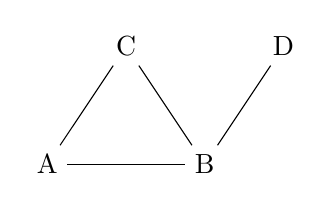
\begin{tikzpicture}

\node (A) at (0,0) {A};
\node (B) at (2,0) {B};
\node (C) at (1,1.5) {C};
\node (D) at (3,1.5) {D};

\draw (A)--(B);
\draw (A)--(C);
\draw (B)--(C);
\draw (B)--(D);

\end{tikzpicture}

\end{center}

\end{frame}

%---------------------------------

\begin{frame}{Bậc của đỉnh}

Bậc của một đỉnh là số cạnh nối với đỉnh đó.

Ví dụ:

\begin{itemize}
\item deg(A) = 2
\item deg(B) = 3
\item deg(C) = 2
\end{itemize}

\end{frame}

%---------------------------------

\begin{frame}{Đường đi và Chu trình}

\textbf{Đường đi (Path)}

\begin{itemize}
\item Là dãy các đỉnh liên tiếp nối với nhau bằng các cạnh
\end{itemize}

\textbf{Chu trình (Cycle)}

\begin{itemize}
\item Là đường đi bắt đầu và kết thúc tại cùng một đỉnh
\end{itemize}

\end{frame}

%---------------------------------

\begin{frame}

\centering
\Huge Cảm ơn!

\end{frame}

\end{document}
